\section{Tecnologías Utilizadas}

Para el desarrollo de este trabajo se utilizaron múltiples herramientas como lo son Git, SublimeText 3, Sublime Merge y los repositorios de Github todo bajo el sistema operativo Ubuntu 20.04.

A continuacion se presentan las herramientas de software de mayor impacto para el desarrollo de este trabajo.

\subsection{Python}

Python es un lenguaje de programación de alto nivel, interpretado y multipropósito. Python es muy utilizado por  la comunidad al ser un leguaje muy fácil de aprender y utilizar por ser un lenguaje de tipado dinámico, además de ser de código abierto.

Python ha tomado popularidad para el desarrollo en deep learning, por su facilidad de uso y la gran variedad de bibliotecas con las que cuenta como TensorFlow, PyTorch, Numpy, Scikit, entre otros.

\subsection{Contenedores Docker}

Un contenedor es una unidad de software que empaqueta el código y todas sus dependencias para que la aplicación se ejecute de forma rápida y confiable de un entorno informático a otro. Una imagen de contenedor de Docker es un paquete de software ligero, independiente y ejecutable que incluye todo lo necesario para ejecutar una aplicación: código, tiempo de ejecución, herramientas del sistema, bibliotecas del sistema y configuraciones \cite{docker2021container}.

La Figura \ref{fig:contenedorDocker} muestra las capas desde la infraestructura hasta los contenendores ejecutandose.

\begin{figure}[H]
    \centering
    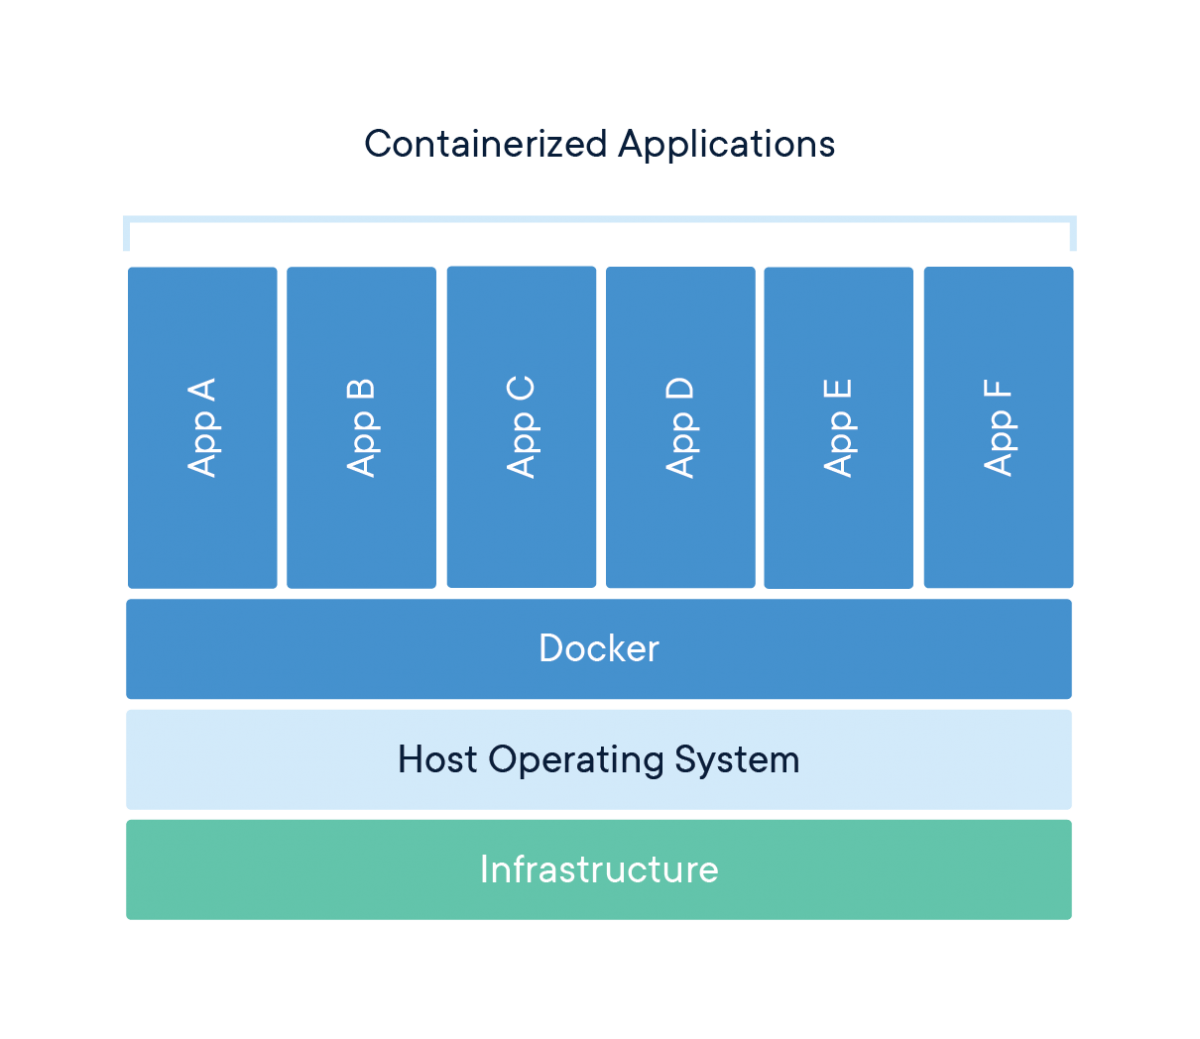
\includegraphics[width=0.6\textwidth]{MarcoTeorico/imgs/container-what-is-container.png}
    \caption{Representacion de un contenedor \cite{docker2021container}.}
    \label{fig:contenedorDocker}
\end{figure}


Docker fue la principal herramienta utilizada para el desarrollo de este trabajo, puesto que, sirvió para replicar múltiples trabajos del estado del arte sin necesidad de complicadas configuraciones al equipo utilizado, además de transferir los experimentos a otro equipo al solo utilizar la imagen creada para este experimento.

\subsection{Nvidia Docker}

NVIDIA Container Toolkit permite crear y ejecutar contenedores acelerados por GPU. Incluye una biblioteca de tiempo de ejecución de contenedores y utilidades para configurar automáticamente los contenedores para aprovechar las GPU de NVIDIA \cite{nvidiaDocker2021overview}.

Nvidia Docker permite la comunicación entre los contenedores de Docker y las GPU de Nvidia en la maquina utilizada como muestra la Figura \ref{fig:nvidiaDocker}.

\begin{figure}[H]
    \centering
    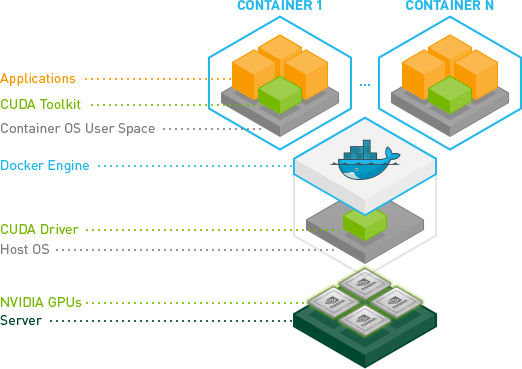
\includegraphics[width=0.6\textwidth]{MarcoTeorico/imgs/nvidia-docker.png}
    \caption{Arquitectura de Nvidia Docker \cite{nvidiaDocker2021overview}.}
    \label{fig:nvidiaDocker}
\end{figure}
